% a-project.tex, v-1.0.3 marcoreis baseado no
% abntex2-modelo-trabalho-academico.tex, v-1.9.7 laurocesar
% Copyright 2012-2018 by abnTeX2 group at http://www.abntex.net.br/ 
% 
% This work consists of the files ........
% 
% -----------------------------------------------------------------------------
% Modelo para desenvolvimento de documentação de projetos acadêmicos
% (tese de doutorado, dissertação de mestrado e trabalhos de monografias em geral) 
% em conformidade com ABNT NBR 14724:2011: Informação e documentação. 
% -----------------------------------------------------------------------------
% Opções para a documentação
%
% Fancy page headings 
%\documentclass[fancyheadings, subook]{Classes/a-prj}
%\documentclass[fancyheadings, sureport]{Classes/a-prj}
%
% Fancy chapters and sections headings 
%\documentclass[fancychapter, subook]{Classes/a-prj}
%\documentclass[fancychapter, sureport]{Classes/a-prj}
%
% Fancy page , chapters and sections headings
%\documentclass[fancyheadings, fancychapter, subook]{Classes/a-prj}
\documentclass[fancyheadings, fancychapter, sureport]{Classes/a-report}
%
% -----------------------------------------------------------------------------
% Alguns comandos para a fancy page headings)
%
% Page header line width
%\footlinewidth{value}
%
% Page footer line width
%\headlinewidth{value}
%
% Page header and footer line width
%\headingslinewidth{value}
%
% Page header and footer lines without text
%\headingslinesonly
%
% The default line width is 0.3pt.
% Set the value to 0pt to remove the page header and/or footer line
%
% -------------------------------------------------------------------------------
% Formato de figuras suportado
% -------------------------------------------------------------------------------
% O formato das figuras depende da forma como o arquivo de saída é gerado.
% As figuras inseridas na pasta Figures serão automaticamente reconhecidas sem
% a necessidade de inserir a extensão do arquivo.
%
% O pdfLaTEX (PDF) suporta figuras com as extensões: pdf, jpg, png e mps.
%
% -------------------------------------------------------------------------------
% Árvore do diretório a-project.tex
%  Diretório
%       \Classes        (requerido)
%       \Figures        (requerido) --------------------------------->
%       \Figures\PDF    (optional)
%       \Figures\JPG    (optional) Figures located within these
%       \Figures\PNG    (optional) folders are searched automatically
%       \Figures\MPS    (optional)  by the a-prj class.
%       \Figures\EPS    (optional)
%       \Figures\PS     (optional) <--------------------------------
%       \Tables         (requerido)
%       \Others         (requerido)
%       \Chapters       (requerido)
%       \Appendices     (optional)
%       \References     (requerido)
%
% -------------------------------------------------------------------------------
% PDF File resumo
\ifpdf
    \hypersetup{
    	backref,
        colorlinks  = true,
        pdftitle    = Modelo de documentação,
        pdfauthor   = {Marco Reis, marco.a.reis@gmail.com},
        pdfsubject  = Mestre em Engenharia,
        pdfcreator  = Subtitulo,
        pdfproducer = PDFLatex,
        pdfkeywords = {documentação, latex, dissertação, tese}}
 \fi
%
% -------------------------------------------------------------------------------
% Relação de pacotes opcionais utilizados
\usepackage[utf8]{inputenc}
\usepackage[brazil]{babel}
\usepackage{longtable}
\usepackage{dcolumn}
\usepackage{multirow}
\usepackage{lscape}
%\usepackage{graphicx}
\usepackage{rotating}
%\usepackage{float,subfigure}
%\usepackage{graphicx, subfigure}
\usepackage{cite}
\usepackage[left=3cm,top=3cm,right=2cm,bottom=2cm]{geometry}
\usepackage[alf]{abntex2cite}
\usepackage{ifpdf}
\usepackage{shadow}
\usepackage{wrapfig}
\usepackage[normalem]{ulem}
\usepackage{makeidx}
\usepackage{yfonts}
\usepackage{algorithm}
\usepackage{algorithmic}
\usepackage{lmodern}
\usepackage[T1]{fontenc}
\usepackage{indentfirst}
\usepackage{color}
\usepackage{microtype}
\usepackage{lipsum}
\usepackage{caption}
\usepackage{subcaption}
\usepackage{plantuml}
\makeindex 
\setlength{\LTcapwidth}{\textwidth}
%
\newtheorem{theorem}{Teorema}
\newtheorem{definition}[theorem]{Definição}
%
% -------------------------------------------------------------------------------
% Configurações do pacote backref
\renewcommand{\backrefpagesname}{Citado na(s) página(s):~}
% Texto padrão antes do número das páginas
\renewcommand{\backref}{}
% Define os textos da citação
\renewcommand*{\backrefalt}[4]{
	\ifcase #1 %
		Nenhuma citação no texto.%
	\or
		Citado na página #2.%
	\else
		Citado #1 vezes nas páginas #2.%
	\fi
}
% 
% -------------------------------------------------------------------------------
% Início do documento raiz
\begin{document}
% Definição do título da página
    \university{Universidade Positivo}
	%\faculty{Programa de...}
	%\school{Escola de...}
% 
    %\course{Engenharia Elétrica}
    \typework{Relatório Final}

    \def\thedegreetitle{Analista de sistemas}
    \def\thefaculty{Escola Politécnica da Universidade Positivo}
    \def\thecourse{Análise e Desenvolvimento de Sistemas}
% 
	%\course{Mestrado em Modelagem Computacional e Tecnologia Industrial}
	%\typework{Disserta\c{c}\~ao de mestrado}
	%\typework{Exame de Qualificação de Mestrado}
% 
	%\course{Engenharia Elétrica}
	%\typework{Tese de doutorado}
	%\typework{Exame de Qualificação de doutorado}
%
% -------------------------------------------------------------------------------
% Informações gerais
    \thesistitle{Portifólio para um profissional em Manutenção Residencial}
    \hidevolume
    \thesisvolume{Volume 1 of 1}
    \thesisauthor{Luciano Diniz}
    \thesisauthorr{Paulo Araujo}
    \thesisauthorrr{Geovany Rodrigues}
    \thesisauthorrrr{James Arruda}
    \thesisauthorrrrr{Diogo de Paula}
    \thesisauthorrrrrr{Jimmy Lovens}
    \thesisadvisor{Prof. Marco Reis, M.Eng.}
    %\hidecoadvisor
    %\thesiscoadvisor{Marco Reis}
    \thesismonthyear{Abril de 2025}
% 
    \maketitlepage
%
% ----------------------------------------------------------------------------
% Inserir Folha de rosto, Nota de estilo, folha de assinaturas, dedicatoria
    \begin{folharosto}

\begin{center}
\theauthor \\
\theauthorr \\
%\theauthorrr \\
%\theauthorrrr \\
%\theauthorrrrr \\
\end{center}
\ \\
\ \\
\ \\
\ \\
\ \\
\begin{spacing}{2}
   \begin{center}
   {\LARGE {\bf \thetitle}}
   \end{center}
\end{spacing}
\ \\
\ \\
\ \\
\vspace*{85mm}
% \begin{flushright}

%    \begin{list}{}{
%       \setlength{\leftmargin}{7.5cm}
%       \setlength{\rightmargin}{0cm}
%       \setlength{\labelwidth}{0pt}
%       \setlength{\labelsep}{\leftmargin}}

%       \item \thetypework apresentada ao \thefaculty, Curso de \thecourse
%       do \theuniversity, como requisito parcial para a obten\c{c}\~ao do
%       t\'itulo de {\bf \thedegreetitle}.

%       \begin{list}{}{
%       \setlength{\leftmargin}{0cm}
%       \setlength{\rightmargin}{0cm}
%       \setlength{\labelwidth}{0pt}
%       \setlength{\labelsep}{\leftmargin}}

%       \item \'Area de conhecimento: Interdisciplinar

%       \item Orientador: \theadvisor
%       \newline \hspace*{2.1cm}  %{\it \theuniversity}

%       \end{list}
%    \end{list}

% \end{flushright}
\ \\
\ \\
\ \\
\ \\
%\begin{spacing}{1.5}
   \begin{center}
   Curitiba \par
   \theuniversity \par
   2025
   \end{center}
%\end{spacing}

\end{folharosto}

    %\begin{notaestilo}
Esta \thetypeworkthree foi elaborada considerando as normas de
estilo (i.e. est\'eticas e estruturais) propostas aprovadas pelo
colegiado do \thefacultytwo e est\~ao dispon\'iveis em formato
eletr\^onico ({\it download} na P\'agina Web
http:$//$ead.fieb.org.br$/$portal\_faculdades$/$dissertacoes-e-teses-mcti.html
ou solicita\c{c}\~ao via e-mail \`a secretaria do
programa) e em formato impresso somente para consulta. \\

Ressalta-se que o formato proposto considera diversos itens das
normas da Associa\c{c}\~ao Brasileira de Normas T\'ecnicas (ABNT),
entretanto opta-se, em alguns aspectos, seguir um estilo pr\'oprio
elaborado e amadurecido pelos professores do programa de
p\'os-gradua\c{c}\~ao supracitado.

\end{notaestilo}

    %\begin{folhaassinaturas}

%\thispagestyle{empty}

\def\signature#1#2{\parbox[b]{1in}{\smash{#1}\vskip12pt}
\hfill \parbox[t]{3in}{\shortstack{\vrule width 3in height
0.4pt\\\small#2}}}

\def\InstituicaoMembro#1#2{\parbox[b]{1in}{\smash{#1}\vskip12pt}
\hfill \parbox[t]{3in}{\shortstack{\vrule width 3in \\\small#2}}}

\def\signaturepage{%

    \begin{spacing}{1.5}
        \begin{center}
        {\LARGE \theuniversity} \\
        {\large \thefaculty} \\
        {\large \thecourse} \\
        \end{center}
    \end{spacing}

   \vskip 0.25in plus 0.4in minus 0.1in

    \begin{spacing}{1.5}
        \begin{sloppypar}
        A Banca Examinadora, constitu\'ida pelos professores abaixo
        listados, leram e recomendam a aprova\c{c}\~ao [com distin\c{c}\~ao] da
        \thetypeworktwo, intitulada ``\thetitle",
        apresentada no dia (dia) de (m\^es) de (ano), como requisito
        parcial para a obten\c{c}\~ao do t\'itulo de {\bf \thedegreetitle}.\\
        \end{sloppypar}
    \end{spacing}

    \def\sigskip{\vskip0.15in plus 0.2in minus 0.1in}
    \def\beginskip{\vskip0.3875in plus 0.2in minus 0.1in}

    \beginskip
    \signature{Orientador:}{Prof. Dr. \theadvisor} \\
    \InstituicaoMembro{}{\theuniversity} \\

    \sigskip
    \beginskip
    \signature{Membro externo da Banca:}{Prof. Dr. Nome completo} \\
    \InstituicaoMembro{}{Institui\c{c}\~ao do membro da banca} \\

    \sigskip
    \beginskip
    \signature{Membro externo da Banca:}{Prof. Dr. Nome completo} \\
    \InstituicaoMembro{}{Institui\c{c}\~ao do membro da banca} \\

    %\sigskip
    %\beginskip
   % \signature{Membro interno da Banca:}{Prof. Dr. Nome completo} \\
   % \InstituicaoMembro{}{Institui��o do membro da banca} \\

    \vfill
    \newpage
    \setcounter{page}{3}
}
%*********************************************************************


\signaturepage


\end{folhaassinaturas}

    %\include{Others/dedicatoria}
    %\include{Others/agradecimentos}
%
% ----------------------------------------------------------------------------
% Resumo/abstract, sumário e siglas
    \begin{romanpagenumbers}
        \begin{thesisresumo}
O presente relatório detalha o processo de desenvolvimento de um portfólio digital para um profissional autônomo na área de manutenção residencial. Em um mercado cada vez mais digitalizado, a presença online tornou-se crucial para a visibilidade e captação de clientes. Este projeto visa suprir a necessidade do cliente em estabelecer uma presença digital robusta, permitindo que potenciais clientes conheçam seus serviços, certificações, experiência e entrem em contato de forma facilitada. O escopo do projeto abrange desde o planejamento estratégico e a definição da identidade visual até a implementação técnica do site, com foco em usabilidade, design responsivo e integração de funcionalidades de contato eficientes. O sucesso deste projeto será medido pela capacidade do portfólio de atrair e converter visitantes em leads qualificados, fortalecendo a marca pessoal do profissional no ambiente digital.
\ \\

% use de três a cinco palavras-chave

\textbf{Palavras-chave}: portfólio digital, manutenção residencial, presença online, captação de clientes, identidade visual.

\end{thesisresumo}

        \begin{thesisabastract}
This report details the development process of a digital portfolio for a freelance professional in home maintenance. In an increasingly digitalized market, an online presence has become crucial for visibility and client acquisition. This project aims to meet the client's need to establish a robust digital presence, allowing potential clients to easily learn about their services, certifications, experience, and contact them. The project scope covers everything from strategic planning and visual identity definition to the technical implementation of the website, focusing on usability, responsive design, and the integration of efficient contact functionalities. The success of this project will be measured by the portfolio's ability to attract and convert visitors into qualified leads, strengthening the professional's personal brand in the digital environment.


\ \\

% use de tr�s a cinco palavras-chave

\textbf{Keywords}: digital portfolio, home maintenance, online presence, client acquisition, visual identity.

\end{thesisabastract}

        % Make list of contents, tables and figures
        \thesiscontents
        \newpage
        %Include other required section
        %\begin{thesisabbreviations}
\begin{footnotesize}
\begin{longtable}[l]{p{2cm}l}
  tprax   \dotfill & \thefaculty \\
  WWW       \dotfill &  World Wide Web \\
\end{longtable}
\end{footnotesize}
\end{thesisabbreviations}

        %\begin{thesissymbols}
\begin{footnotesize}
\begin{longtable}[l]{p{2cm}l}
  $\partial$   \dotfill  & Bla bla bla \\
  $\prod$       \dotfill & ble ble ble \\
  $\partial$   \dotfill  & Bla bla bla \\
  $\prod$       \dotfill & ble ble ble \\
  $\partial$   \dotfill  & Bla bla bla \\
  $\prod$       \dotfill & ble ble ble \\
  $\partial$   \dotfill  & Bla bla bla \\
  $\prod$       \dotfill & ble ble ble \\
  $\partial$   \dotfill  & Bla bla bla \\
  $\prod$       \dotfill & ble ble ble \\
  $\partial$   \dotfill  & Bla bla bla \\
  $\prod$       \dotfill & ble ble ble \\
  $\partial$   \dotfill  & Bla bla bla \\
  $\prod$       \dotfill & ble ble ble \\
  $\partial$   \dotfill  & Bla bla bla \\
  $\prod$       \dotfill & ble ble ble \\
  $\partial$   \dotfill  & Bla bla bla \\
  $\prod$       \dotfill & ble ble ble \\
  $\partial$   \dotfill  & Bla bla bla \\
  $\prod$       \dotfill & ble ble ble \\
  $\partial$   \dotfill  & Bla bla bla \\
  $\prod$       \dotfill & ble ble ble \\
  $\partial$   \dotfill  & Bla bla bla \\
  $\prod$       \dotfill & ble ble ble \\
  $\partial$   \dotfill  & Bla bla bla \\
  $\prod$       \dotfill & ble ble ble \\
  $\partial$   \dotfill  & Bla bla bla \\
  $\prod$       \dotfill & ble ble ble \\
  $\partial$   \dotfill  & Bla bla bla \\
  $\prod$       \dotfill & ble ble ble \\
  $\partial$   \dotfill  & Bla bla bla \\
  $\prod$       \dotfill & ble ble ble \\
  $\partial$   \dotfill  & Bla bla bla \\
  $\prod$       \dotfill & ble ble ble \\
  $\partial$   \dotfill  & Bla bla bla \\
  $\prod$       \dotfill & ble ble ble \\
  $\partial$   \dotfill  & Bla bla bla \\
  $\prod$       \dotfill & ble ble ble \\          
\end{longtable}
\end{footnotesize}
\end{thesissymbols}

        %Switch the page numbering back to the default format
    \end{romanpagenumbers}
%
% ---------------------------------------------------------------------------
% Include thesis chapters
    \parskip=\baselineskip
    \chapter{Introdução}
\label{chap:intro}

% Este pode ser um parágrafo citado por alguém \cite{Barabasi2003-1} e \cite{barabasi2003linked}.
% Para ajustar veja o comentário do capítulo \ref{chap:fundteor}.

% As orientações do robô \cite{aperea-1}.

% fakdfjlsdjfldsjfldsj
% dfkhfdskfhkdjh


% Segundo \citeonline{barabasi2003linked}, ...

% 
% \loremipsum dolor sit amet, consectetur adipiscing elit. Sed do eiusmod tempor incididunt ut labore et dolore magna aliqua. Ut enim ad minim veniam, quis nostrud exercitation ullamco laboris nisi ut aliquip ex ea commodo consequat. Duis aute irure dolor in reprehenderit in voluptate velit esse cillum dolore eu fugiat nulla pariatur. Excepteur sint occaecat cupidatat non proident, sunt in culpa qui officia deserunt mollit anim id est laborum.
%--------- NEW SECTION ----------------------
\section{Objetivos}
\label{sec:obj}
Este projeto consiste em desenvolver um robô bípede de pequeno porte, ou seja que se desloca sobre dois pés. O robô deve ser capaz de se locomover e desviar de obstáculos em um determinado ambiente. 
\label{sec:obj}

\subsection{Objetivos Específicos}
\label{ssec:objesp}
Os objetivos específicos deste projeto são:
\begin{itemize}
      \item Desenvolver habilidades de gestão de projetos.
      \item Desenvolver algoritmos utilizando ROS;
      \item Utilizar visão computacional;
      \item Simular um robô no gazebo;
  \end{itemize}

\subsubsection*{Objetivos específicos principais}
\label{sssec:obj-principais}
ok vendo Aqui


\begin{equation}
  E=mc
\end{equation}


\begin{equation*}
  m=\frac{E}{c}
\end{equation*}

\begin{equation}
  m=E/c
\end{equation}


%--------- NEW SECTION ----------------------
\section{Justificativa}
\label{sec:justi}

O pesquisador/estudante deve apresentar os aspectos mais
relevantes da pesquisa ressaltando os impactos (e.g. cient\'ifico,
tecnol\'ogico, econ\^omico, social e ambiental) que a pesquisa
causar\'a. Deve-se ter cuidado com a ingenuidade no momento em que
os argumentos forem apresentados.




%--------- NEW SECTION ----------------------
\section{Organização do documento}
\label{section:organizacao}

Este documento apresenta $5$ capítulos e está estruturado da seguinte forma:

\begin{itemize}

  \item \textbf{Capítulo \ref{chap:intro} - Introdução}: Contextualiza o âmbito, no qual a pesquisa proposta está inserida. Apresenta, portanto, a definição do problema, objetivos e justificativas da pesquisa e como este \thetypeworkthree está estruturado;
  \item \textbf{Capítulo \ref{chap:fundteor} - Fundamentação Teórica}: XXX;
  \item \textbf{Capítulo \ref{chap:metod} - Materiais e Métodos}: XXX;
  \item \textbf{Capítulo \ref{chap:result} - Resultados}: XXX;
  \item \textbf{Capítulo \ref{chap:conc} - Conclusão}: Apresenta as conclusóes, contribuições e algumas sugestões de atividades de pesquisa a serem desenvolvidas no futuro.

\end{itemize}

    \chapter{Conceito do projeto do portfólio}
\label{chap:fundteor}
%--------- NEW SECTION ----------------------
Os robôs móveis têm a capacidade de se moverem sem a assistência de um operador humano. Os mesmos podem ser classificados,quanto ao sistema de locomoção, como terrestres, aquáticos e aéreos. Os terrestres são subdivididos em robôs que possuem rodas, pernas (bípedes) ou esteiras (ref:Review ArticleA review of mobile robots:). Cada um desses métodos possuem características especifícas quanto ao movimento a ser realizado. Os bípedes, por exemplo, simulam um caminhar antropomórfico, semelhante aos humanos.
% isso é igual <=  === <> #{ #( www
% <| |>
% ===

Lista dos documentos
\begin{enumerate}
   \item diagrama de classe
   \item diagrama de casos de uso
   \item diagrama de sequência
\end{enumerate}

O desenvolvimento deste projeto consiste em produzir um robô que possa caminhar sobre duas pernas. Além disso, o walker deve se locomover de forma autonôma a fim de realizar uma dada missão.

Neste capítulo serão abordados os requisitos do cliente, os requisistos técnicos, a missão do robô e a pesquisa por similares. 



%conferir se precisa de requisitos do cliente
\section{Requisitos do cliente}
 O cliente definiu certos requisitos quanto à operação e  às características do robô:
 \begin{itemize}
    \item Operar em uma área de 2x1,5m;
    \item Possuir uma altura de aproximadamente 30 cm;
    \item Ser capaz de operar por, no mínimo 20 minutos;
    \item Ser capaz de desviar de obstáculos;
 \end{itemize}

 \section{Requisitos funcionais}

\lipsum[2-4]

%  \section{Missão}
%  \lipsum
%  %desenvolver mais
%  Além disso, o Walker deve realizar um desafio, que consiste em navegar de forma autônoma, se localizar por meio de tags e encontrar um determinado objeto.



%  \section{Pesquisa por similares}


% %----------------------------------------------------------

% %--------- NEW SECTION ----------------------


% %---------------picture------------------------------------
% % \begin{figure}
% %     \centering
% %     \subfigure[Figure A]{\label{fig:a}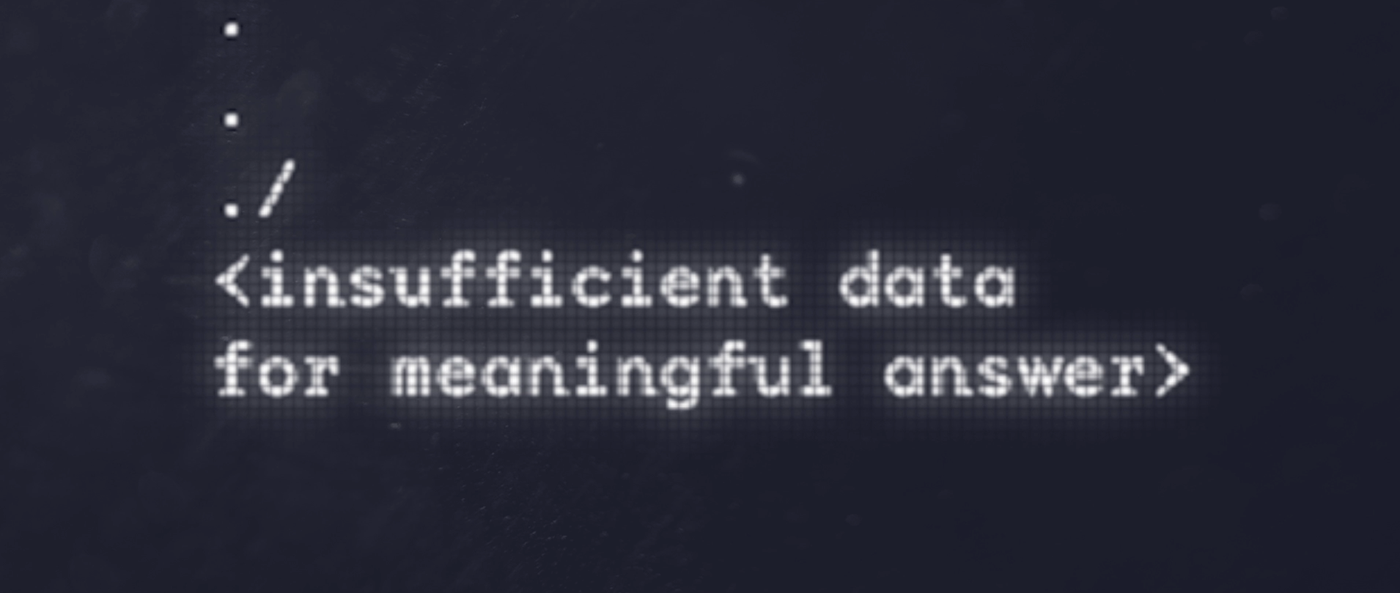
\includegraphics[width=60mm]{./lq}}
% %     \subfigure[Figure B]{\label{fig:b}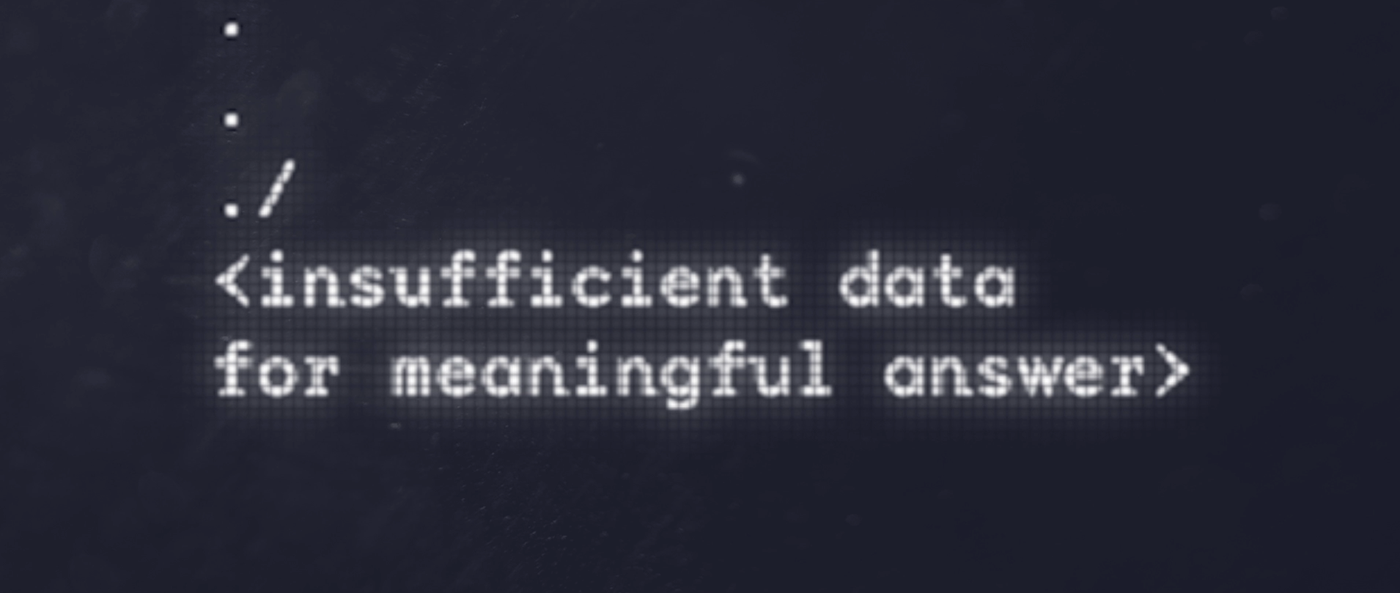
\includegraphics[width=60mm]{./lq}}
% %     \subfigure[Figure C]{\label{fig:c}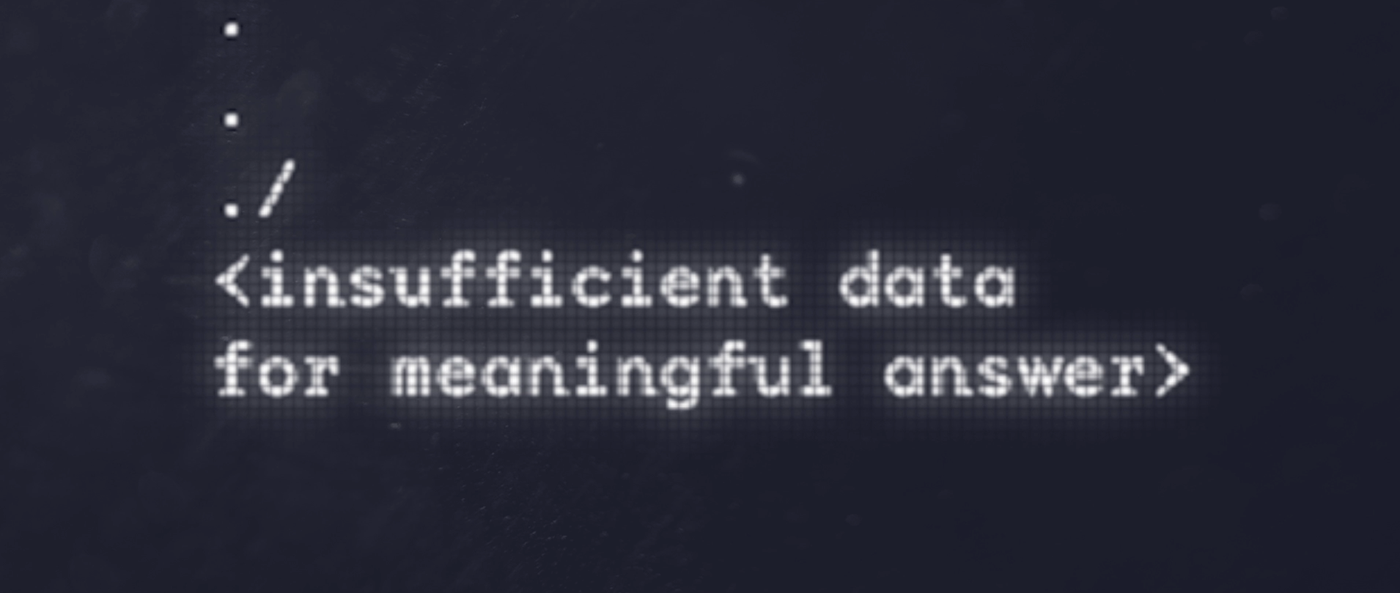
\includegraphics[width=\textwidth]{./lq}}
% %     \caption{Three simple graphs}
% %     \label{fig:three graphs}
% % \end{figure}
% %----------------------------------------------------------

% % \begin{figure}
% %     \centering
% %     \begin{subfigure}[b]{0.3\textwidth}
% %         \centering
% %         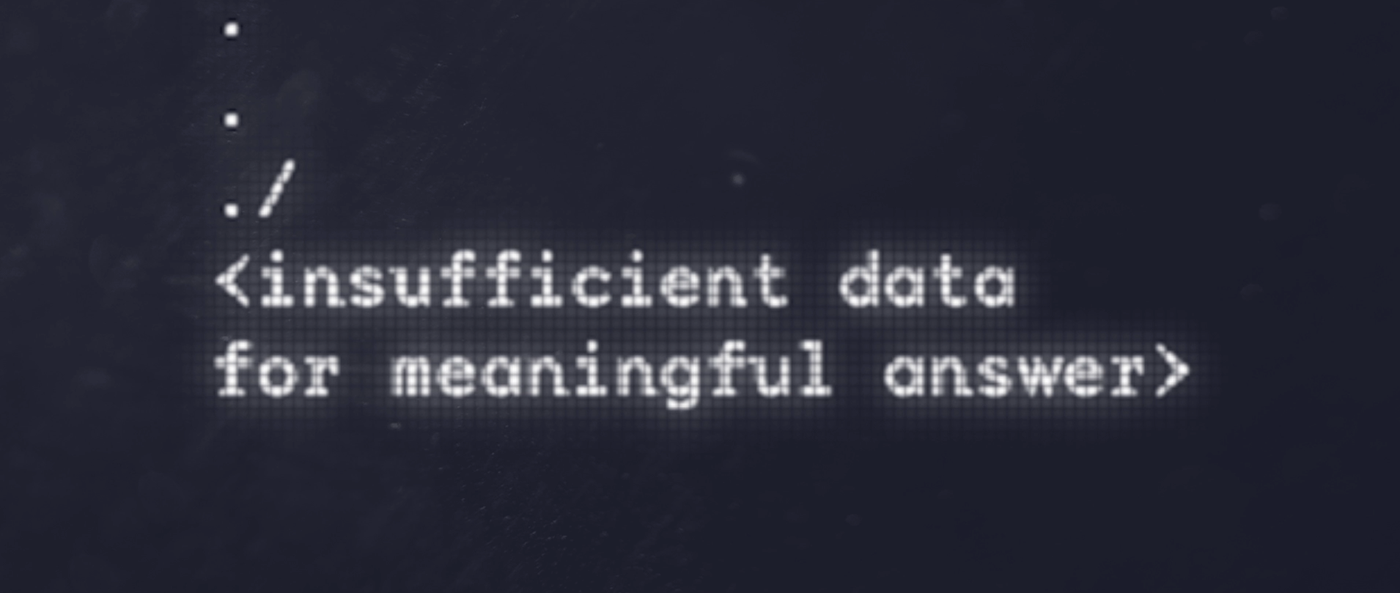
\includegraphics[width=\textwidth]{./lq}
% %         \caption{$y=x$}
% %         \label{fig:y equals x}
% %     \end{subfigure}
% %     \hfill
% %     \begin{subfigure}[b]{0.3\textwidth}
% %         \centering
% %         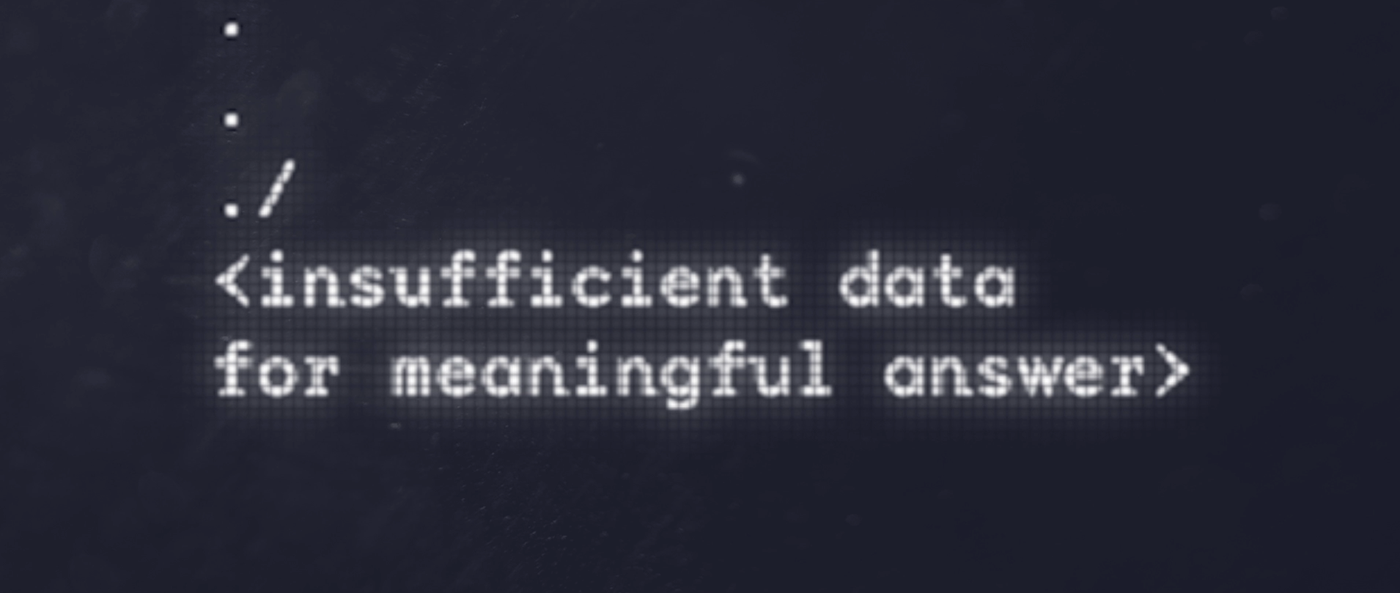
\includegraphics[width=\textwidth]{./lq}
% %         \caption{$y=3sinx$}
% %         \label{fig:three sin x}
% %     \end{subfigure}
% %     \hfill
% %     \begin{subfigure}[b]{0.3\textwidth}
% %         \centering
% %         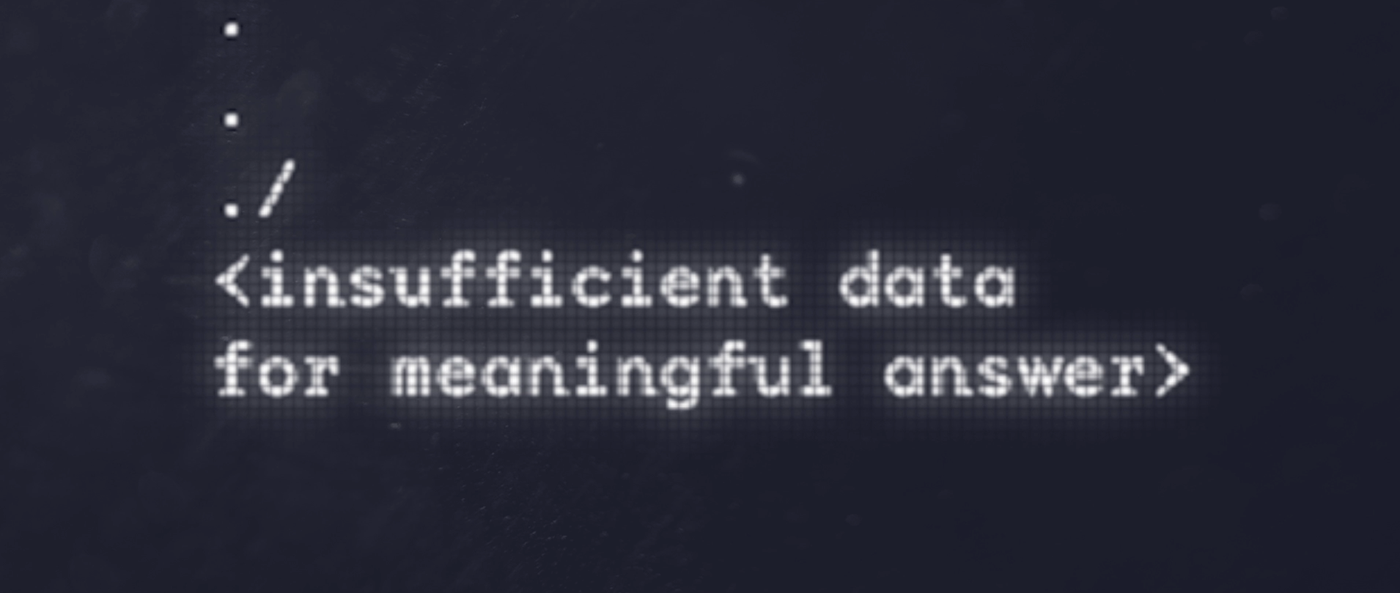
\includegraphics[width=\textwidth]{./lq}
% %         \caption{$y=5/x$}
% %         \label{fig:five over x}
% %     \end{subfigure}
% %        \caption{Three simple graphs}
% %        \label{fig:three graphs}
% % \end{figure}


% % %--------- NEW SECTION ----------------------
% % \section{Assunto 2}
% % \label{sec:ass2}
% % flkjasdlkfjasdlkfjs

% % \begin{table}[h]
% %     \begin{subtable}[h]{0.45\textwidth}
% %         \centering
% %         \begin{tabular}{l | l | l}
% %         Day & Max Temp & Min Temp \\
% %         \hline \hline
% %         Mon & 20 & 13\\
% %         Tue & 22 & 14\\
% %         Wed & 23 & 12\\
% %         Thurs & 25 & 13\\
% %         Fri & 18 & 7\\
% %         Sat & 15 & 13\\
% %         Sun & 20 & 13
% %        \end{tabular}
% %        \caption{First Week}
% %        \label{tab:week1}
% %     \end{subtable}
% %     \hfill
% %     \begin{subtable}[h]{0.45\textwidth}
% %         \centering
% %         \begin{tabular}{l | l | l}
% %         Day & Max Temp & Min Temp \\
% %         \hline \hline
% %         Mon & 17 & 11\\
% %         Tue & 16 & 10\\
% %         Wed & 14 & 8\\
% %         Thurs & 12 & 5\\
% %         Fri & 15 & 7\\
% %         Sat & 16 & 12\\
% %         Sun & 15 & 9
% %         \end{tabular}
% %         \caption{Second Week}
% %         \label{tab:week2}
% %      \end{subtable}
% %      \caption{Max and min temps recorded in the first two weeks of July}
% %      \label{tab:temps}
% % \end{table}
    \chapter{Desenvolvimento do projeto}
\label{chap:metod}
 Nesta seção, serão apresentados os métodos e processos utilizados para o desenvolvimento do portfólio digital, incluindo a metodologia adotada, a arquitetura geral do sistema, os requisitos técnicos e a modelagem dos processos. O objetivo é fornecer uma visão clara e estruturada das etapas envolvidas na criação do portfólio, desde a concepção até a implementação.

\subsection{Metodologia do projeto}
    A metodologia adotada para o desenvolvimento deste portfólio digital é baseada no modelo ágil, que prioriza a flexibilidade, a colaboração e a entrega incremental de valor. O processo foi dividido em etapas, começando com o levantamento de requisitos, seguido pela modelagem do sistema, prototipagem e testes. Essa abordagem permite uma adaptação rápida às mudanças nas necessidades do cliente e garante que o produto final atenda às expectativas.

\subsubsection{Gerenciamento Ágil de Projetos}
O gerenciamento ágil, inspirado no framework Scrum~ \cite{schwaber2001agile}, orientou o andamento do projeto. A plataforma Trello foi utilizada para acompanhamento das atividades em sprints quinzenais.

\subsubsection{Engenharia de Requisitos}

 De acordo com Sommerville~\cite{kotonya1998requirements}, a engenharia de requisitos é uma etapa fundamental no desenvolvimento de software, pois envolve a identificação, análise e documentação das necessidades do cliente. No caso deste portfólio digital, foram realizadas reuniões com o cliente para entender suas expectativas e requisitos funcionais e não funcionais. A partir dessas informações, foi possível elaborar um documento de requisitos que serviu como base para as etapas seguintes do projeto.

\section{Ideação}
%escrever oq sera apresentado

A fase de ideação foi crucial para o desenvolvimento do portfólio digital, onde foram levantadas as necessidades e expectativas do cliente. A equipe realizou reuniões com o cliente para entender suas demandas, preferências estéticas e funcionais, além de analisar portfólios digitais similares no mercado. Essa etapa inicial permitiu a definição clara dos objetivos do projeto e a identificação dos requisitos essenciais.

\subsection{Arquitetura Geral}
 A estrutura da arquitetura do portfólio digital foi concebida para ser intuitiva e responsiva, garantindo uma experiência de usuário fluida em diferentes dispositivos. A camada de apresentação é responsável pela interface do usuário. Dando a ela um design responsivo, utilizando HTML e CSS para a estrutura e estilo, respectivamente. O JavaScript foi integrado para adicionar interatividade e dinamismo à interface como algumas animações.

\begin{figure}[H]
    \centering
    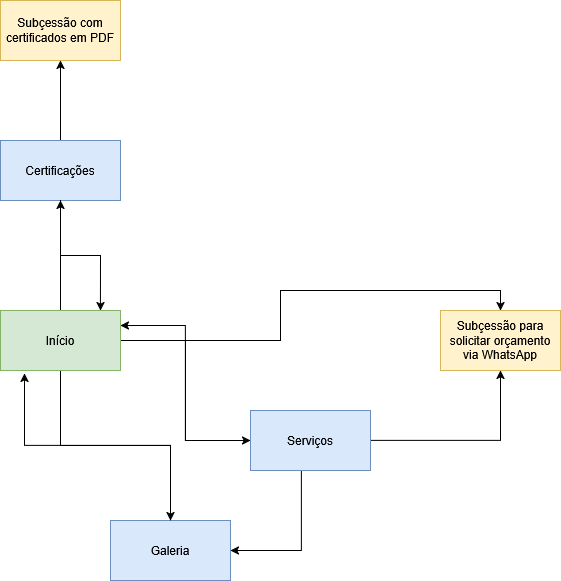
\includegraphics[width=0.6\textwidth]{Figures/arquitetura.png} % use your image path and name here
    \caption{Arquitetura.}
    \label{fig:Arquitetura}
\end{figure}

Neste conjunto se encontram as páginas principais do portfólio, como a página inicial, a seção de projetos e a página de contato.

\subsection{Requisitos técnicos}

Os requisitos técnicos foram definidos com base nas necessidades do cliente e nas melhores práticas de desenvolvimento web. A seguir, estão os principais requisitos:
\begin{itemize}
    \item \textbf{Tecnologias Utilizadas:} HTML, CSS e JavaScript.
    \item \textbf{Funcionalidades:} O portfólio deve incluir uma página inicial, uma seção de projetos, uma página de contato e uma seção de certificados.
    \item \textbf{Responsividade:} O design deve ser responsivo, adaptando-se a diferentes tamanhos de tela, incluindo dispositivos móveis e desktops.
    \item \textbf{Desempenho:} O site deve carregar rapidamente e ser otimizado para uma boa performance, mesmo em conexões lentas.
    \item \textbf{Manutenção:} O código deve ser bem documentado e organizado, facilitando futuras manutenções e atualizações.
\end{itemize}

%desdobramento da função qualidade
\subsection{Quality Function Deployment}

O QFD (Quality Function Deployment) foi utilizado para garantir que as necessidades do cliente fossem traduzidas em requisitos técnicos claros e mensuráveis. Através de uma matriz QFD, foram identificadas as prioridades do cliente e como elas se relacionam com as características do sistema. Essa abordagem ajudou a alinhar as expectativas do cliente com as funcionalidades do portfólio digital.

 \begin{figure} [H]	
     \centering
     \caption{ Primeiro ciclo QFD}
     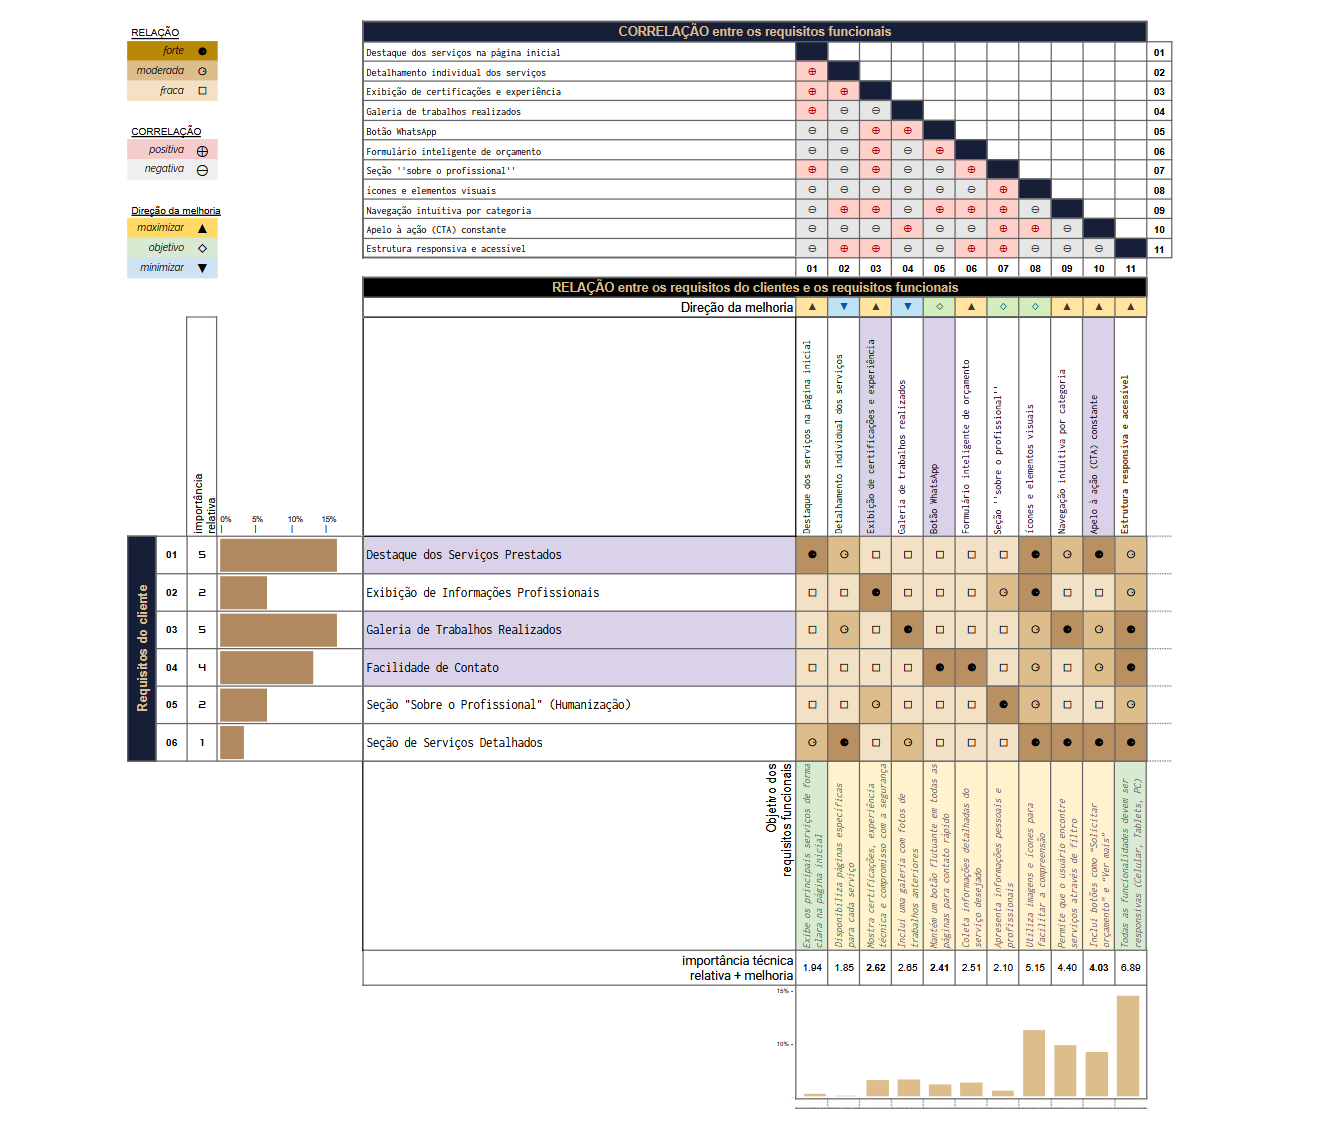
\includegraphics[width=0.8\textwidth]{Figures/matrizqfd.png}
     \caption*{Matriz-QFD}
     \label{fig:QFD}
\end{figure}
   

% % %--------- NEW SECTION ----------------------
% % \section{Interface do Usuário}
% % \label{sec:ui}
% % \lipsum[1]

% % %--------- NEW SECTION ----------------------
% % \section{Simulação do sistema}
% % \label{sec:sim}
% % \lipsum[2-4]
\subsection{Modelagem dos processos}

 O BPMN (Business Process Model and Notation) foi utilizado para modelar os processos envolvidos no desenvolvimento do portfólio digital. Essa abordagem permitiu uma visualização clara dos fluxos de trabalho, facilitando a identificação de etapas críticas e a otimização dos processos. A modelagem BPMN também ajudou a garantir que todos os membros da equipe estivessem alinhados quanto às responsabilidades e prazos.


Essas informações advieram do modelo esquematico de processos, no qual consultamos o cliente para entender suas necessidades e expectativas.

\begin{figure}[H]
    \centering
    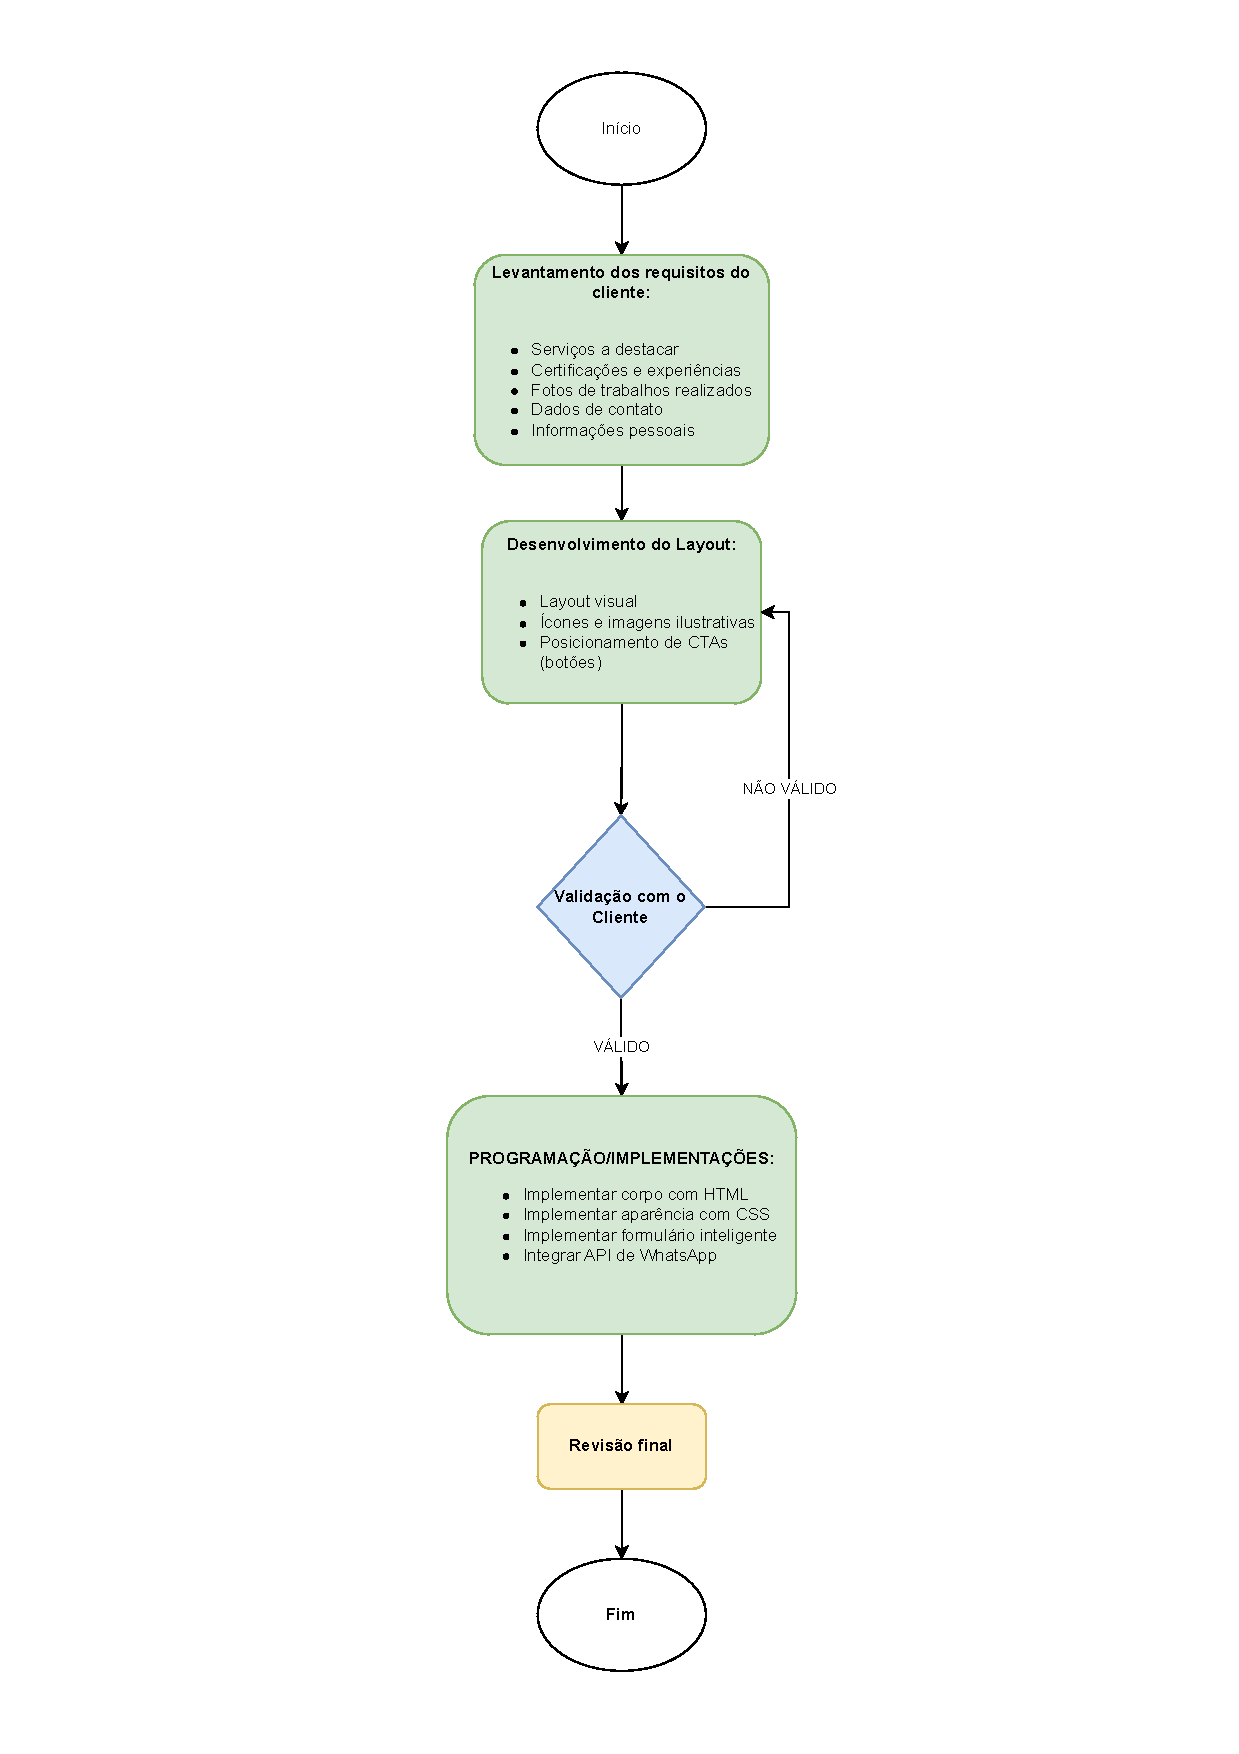
\includegraphics[width=0.6\textwidth]{Figures/modelo_esquematico_de_processos..pdf} % use your image path and name here
    \caption{Modelo esquemático de processos.}
    \label{fig:esquema}
\end{figure}





    \chapter{Resultados}
\label{chap:result}

O desenvolvimento do portfólio digital resultou em um produto funcional e alinhado às expectativas do cliente. A seguir, são apresentados os principais resultados alcançados durante o projeto.

% %--------- NEW SECTION ----------------------
% \section{Testes unitários}
% \label{sec:testu}
% \lipsum[1]

% \section{Integração do sistema}
% \label{sec:intsis}
% \lipsum[1]

% %--------- NEW SECTION ----------------------
% \section{Testes integrados}
% \label{sec:testi}
% \lipsum[1]

\section{Diagrama de classes}
\label{sec:class}
O diagrama de classes é uma representação visual das classes do sistema e seus relacionamentos. Ele é utilizado para descrever a estrutura do sistema e como as classes interagem entre si. A Figura \ref{fig:diagrama-classes} apresenta o diagrama de classes do sistema desenvolvido.

\begin{figure}[H]
    \centering
    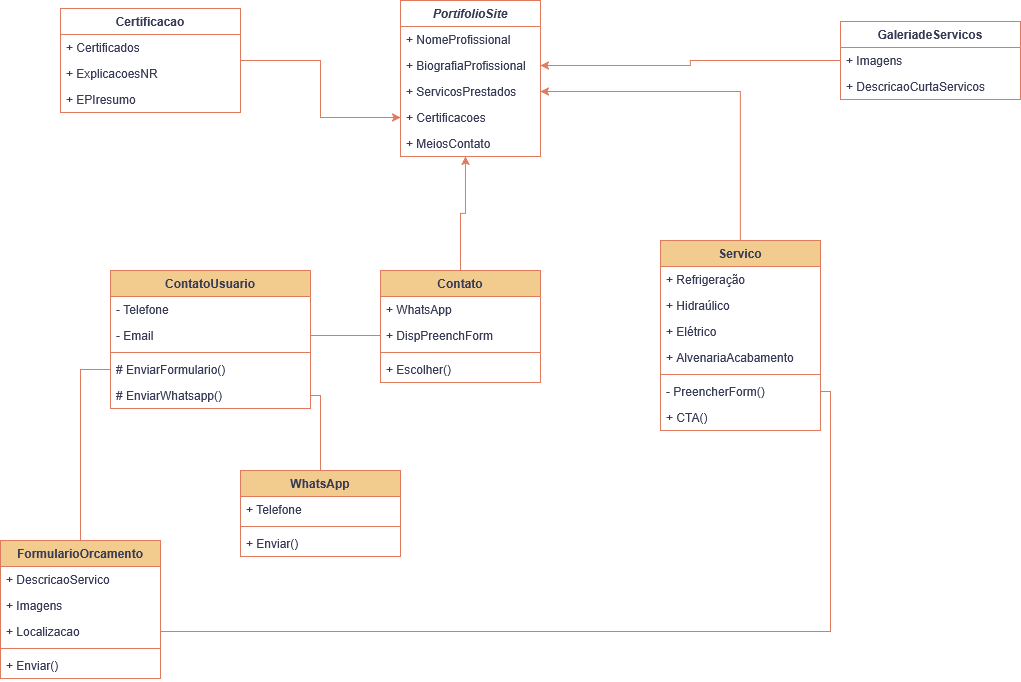
\includegraphics[width=0.6\textwidth]{Figures/Diagrama_de_classes.png} % use your image path and name here
    \caption{Diagrama de classes.}
    \label{fig:diagrama-classes}
\end{figure}

\section{Diagrama de casos de uso}
\label{sec:casos}
O diagrama de casos de uso é uma representação visual das funcionalidades do sistema e como os usuários interagem com ele. Ele é utilizado para descrever os requisitos funcionais do sistema e identificar os atores envolvidos. A Figura \ref{fig:diagrama-uso} apresenta o diagrama de casos de uso do sistema desenvolvido.

\begin{figure}[H]
    \centering
    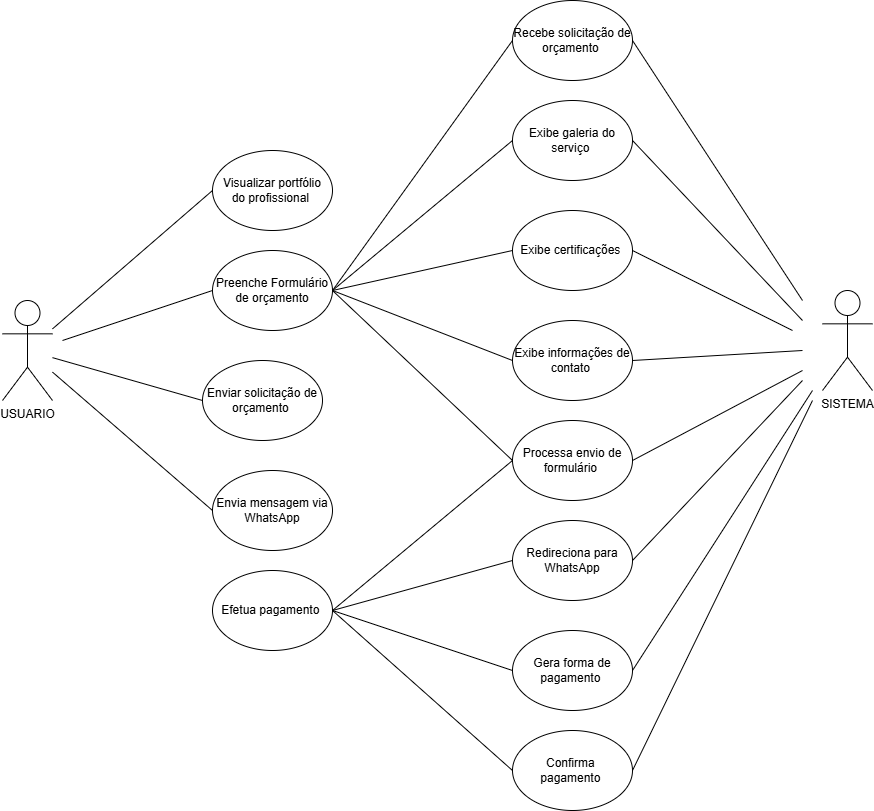
\includegraphics[width=0.6\textwidth]{Figures/Diagrama_de_uso.png} % use your image path and name here
    \caption{Diagrama de casos de uso.}
    \label{fig:diagrama-uso}
\end{figure}


\section{Diagrama de sequência}
\label{sec:sequencia}   
O diagrama de sequência é uma representação visual das interações entre os objetos do sistema ao longo do tempo. Ele é utilizado para descrever o fluxo de mensagens entre os objetos e como eles colaboram para realizar uma funcionalidade específica. A Figura \ref{fig:diagrama-sequencia} apresenta o diagrama de sequência do sistema desenvolvido.

\begin{figure}[H]
    \centering
    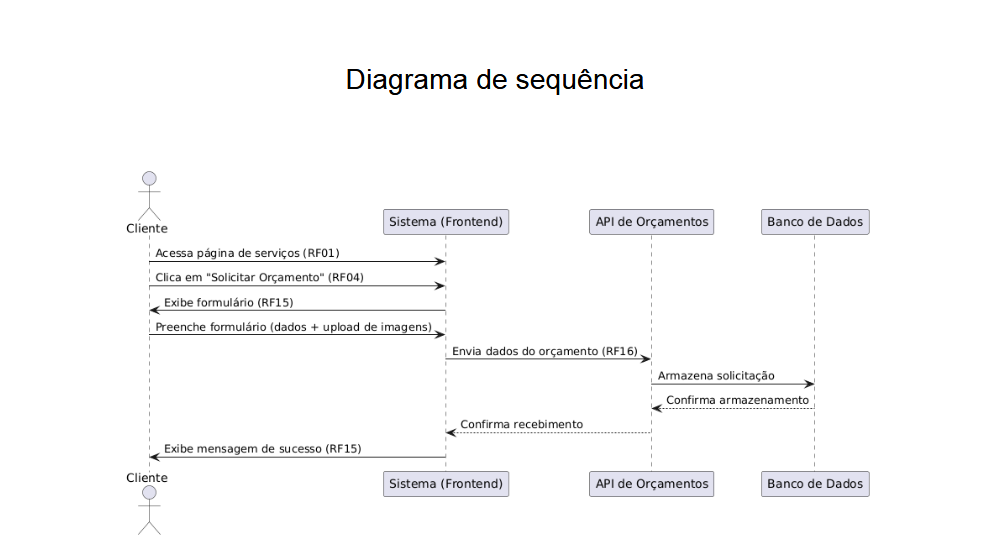
\includegraphics[width=0.6\textwidth]{Figures/seq.png} % use your image path and name here
    \caption{Diagrama de sequência.}
    \label{fig:diagrama-sequencia}
\end{figure}

O cliente inicia o processo acessando a página onde os serviços são destacados e, em seguida, clica no botão "Solicitar Orçamento". Ao realizar essa ação, é apresentado um formulário inteligente, no qual o sistema exibe campos para que o cliente possa inserir a descrição do serviço, fazer o upload de imagens e informar a localização. Após o cliente preencher e enviar esses dados, ocorre a integração com uma API: o sistema envia as informações para a API de orçamentos, que pode ser tanto do WhatsApp quanto uma API independente. Essa API, por sua vez, armazena os dados recebidos no banco de dados e retorna uma confirmação. Como feedback, o sistema exibe uma mensagem de sucesso para o cliente, finalizando a solicitação.











    \chapter{Conclusão}
\label{chap:conc}

A conclus\~ao deste trabalho apresenta uma vis\~ao geral do
desenvolvimento do port\'ifolio digital, destacando as etapas
realizadas, os resultados alcançados e as li\c{c}\~oes aprendidas ao longo do processo. O objetivo principal foi criar uma plataforma que atenda \`a necessidade do cliente de estabelecer uma identidade digital profissional, utilizando boas pr\'aticas de análise e projeto de software.



\section{Considerações finais}
\label{sec:consid}

O desenvolvimento do portfólio digital para o profissional de manutenção residencial foi um processo enriquecedor, que envolveu a aplicação de conceitos teóricos e práticos de Análise e projeto de Software. Através das etapas de ideação, simulação do sistema, design da interface do usuário e testes, foi possível criar uma solução que não apenas atende às necessidades do cliente, mas também se destaca pela sua funcionalidade e estética.

    % include more chapters ...
%
% ----------------------------------------------------------------------------
% Include thesis appendices
        %% Thesis Appendix -------------------------------------------------------

\chapter{Logbook}
\label{Append:log}




%
% ----------------------------------------------------------------------------
% Configurar as referencias bibliograficas
	\renewcommand\bibname{Referências}
    \addcontentsline{toc}{chapter}{Referências}
    \bibliography{References/referencias}
%
% ----------------------------------------------------------------------------
% Finishing him
    \include{Others/ultimafolha}
\end{document}
%
% -------------------------------------------------------------------------------
% Aqui termina a formatação para o documento.
% In God We Trust. All Other Bring Data. 
%
% -------------------------------------------------------------------------------